% Presentation 3 — Answer Key Evaluation DEP
% Narrative: scope -> UI -> APIs -> persistence/config -> auth -> AI transports
%          -> objective pipeline -> code-eval (+ LeetCode) -> Drive/Sheets
%          -> ZIP/PDF + Sheets publishing + Evaluate UI
%          -> throughput/fuzzy/API contracts -> OCR reference -> supplemental coverage -> closing
% pdflatex presentation3_future_development.tex (run twice for stable outlines)
\documentclass[aspectratio=169]{beamer}

\usetheme{Madrid}
\usepackage[T1]{fontenc}
\usepackage[utf8]{inputenc}
\usepackage{lmodern}
\usepackage{hyperref}
\usepackage{booktabs}
\usepackage{multicol}
\usepackage{tikz}
\usetikzlibrary{arrows.meta, positioning}

\usepackage{listings}
\usepackage{xcolor}

\definecolor{cg}{RGB}{0,110,80}
\definecolor{cgray}{RGB}{100,100,100}

\newcommand{\codesmall}{\ttfamily\footnotesize}

\lstdefinestyle{py}{
  language=Python,
  basicstyle=\ttfamily\tiny,
  keywordstyle=\color{blue}\bfseries,
  commentstyle=\color{cg}\itshape,
  stringstyle=\color{orange},
  numbers=left,
  numberstyle=\tiny\color{cgray},
  breaklines=true,
  frame=single,
  tabsize=2,
}
\lstdefinestyle{pys}{
  language=Python,
  basicstyle=\ttfamily\scriptsize,
  keywordstyle=\color{blue}\bfseries,
  commentstyle=\color{cg}\itshape,
  breaklines=true,
  frame=single,
  tabsize=2,
}
\lstdefinestyle{jsx}{
  basicstyle=\ttfamily\tiny,
  keywordstyle=\color{blue}\bfseries,
  breaklines=true,
  frame=single,
  keywords={const,async,await,import,export,from,if,return,try,catch},
}

\title[Presentation 3]{Answer Key Evaluation DEP}
\subtitle{Unified technical overview --- one source file, one PDF}
\author{Project documentation deck}
\date{\today}

\begin{document}

\begin{frame}\titlepage\end{frame}

\section{Introduction}

\begin{frame}{Outline (matches section order)}
  \small
  \begin{enumerate}
    \item \textbf{Introduction} --- repository layout and system diagram.
    \item \textbf{Frontend} --- React/Vite atlas and representative code.
    \item \textbf{Backend and APIs} --- routers, REST surface, domain models, objective ingress paths.
    \item \textbf{Persistence and configuration} --- SQLite, cache keys, Supabase pool, migrations, environment variables.
    \item \textbf{Authentication} --- Supabase vs FastAPI boundary.
    \item \textbf{Gemini and Vertex} --- how vision and text models are invoked (objective + code paths).
    \item \textbf{Objective grading pipeline (services)} --- TikZ chain + module cheat-sheet (after Gemini overview).
    \item \textbf{Code evaluation} --- C-from-image, gcc, syntax repair; then \textbf{LeetCode testcase library}.
    \item \textbf{Google Drive and Sheets} --- integration snippets.
    \item \textbf{ZIP, PDF, Sheets publishing, and Evaluate UI} --- multipart ZIP/PDF uploads, page splitting and synthetic IDs, master/marks/response/Super tabs, export endpoints, React evaluate page modes and toolbar.
    \item \textbf{Throughput, fuzzy matching, and HTTP contracts} --- batch load shaping (token buckets, dual OCR), streaming pipeline, Sheets fuzzy roster logic, Drive rename templates, Pydantic/multipart API surfaces.
    \item \textbf{OCR and migrations reference} --- tuning knobs and DDL (cross-reference to persistence).
    \item \textbf{Supplemental repository coverage} --- scoring internals, answer-key parsers, Drive/CLI/offline OCR, pipeline SQLite, Fly/Railway deploy, tests/fixtures, markdown docs.
    \item \textbf{Closing} --- screenshots placeholders, themes, future work, build.
  \end{enumerate}
  \vfill
  \footnotesize All content is in this \texttt{.tex} file only; there is no companion slide deck.
\end{frame}

\begin{frame}[t]{How to read this deck}
  \small
  \begin{itemize}
    \item \textbf{Objective grading}: ZIP, Drive folder, or PDF $\rightarrow$ OCR $\rightarrow$ answer-key match $\rightarrow$ SQLite/cache $\rightarrow$ optional Sheets/Drive rename.
    \item \textbf{Code grading}: separate HTTP prefix \texttt{/api/code-eval/}; shares Gemini patterns but uses \texttt{c\_code\_evaluator} + LeetCode-shaped tests.
    \item Later slides follow section order: persistence/config $\rightarrow$ auth $\rightarrow$ Gemini $\rightarrow$ objective pipeline $\rightarrow$ code-eval (including LeetCode) $\rightarrow$ Drive/Sheets $\rightarrow$ ZIP/PDF + Sheets publishing + Evaluate UI $\rightarrow$ throughput/fuzzy/API contracts $\rightarrow$ OCR reference $\rightarrow$ supplemental coverage $\rightarrow$ closing.
  \end{itemize}
\end{frame}

\begin{frame}{Top-level repository layout}
  \footnotesize
  \begin{tabular}{@{}p{4.2cm}p{9.4cm}@{}}
    \toprule
    Path & Purpose \\
    \midrule
    \texttt{frontend-new-design/} & Vite React SPA: Supabase Auth + UI; calls FastAPI via \texttt{VITE\_BACKEND\_URL}. \\
    \texttt{backend/} & FastAPI \texttt{main.py}; routers \texttt{api/endpoints.py}, \texttt{batch\_endpoints\_optimized.py}, \texttt{code\_eval\_endpoints.py}. \\
    \texttt{backend/services/*.py} & Drive, Sheets, OCR variants, evaluation, cache, PDF split, DB pool, etc. \\
    \texttt{backend/migrations/*.sql} & Supabase DDL for \texttt{result\_cache}, \texttt{pdf\_page\_map}. \\
    \texttt{c\_code\_evaluator/} & Image$\rightarrow$C code (Gemini); compile-fix; LeetCode harness (\texttt{leetcode\_mode.py}). \\
    \bottomrule
  \end{tabular}
\end{frame}

\begin{frame}{End-to-end system context (single product)}
  \centering
  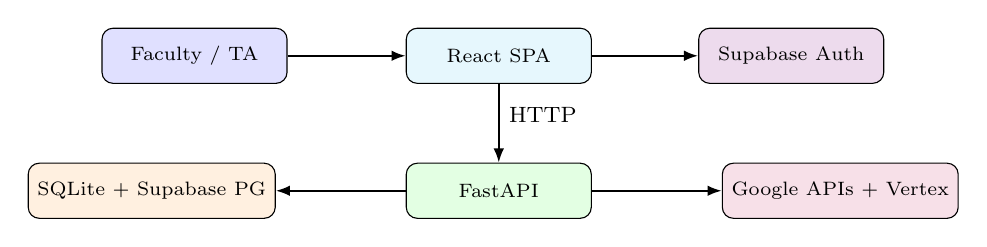
\begin{tikzpicture}[font=\scriptsize,
    box/.style={draw,rounded corners,minimum width=2.35cm,minimum height=0.7cm,align=center},
    arr/.style={-{Latex[length=1.8mm]},thick}]
    \node[box,fill=blue!12](u){Faculty / TA};
    \node[box,fill=cyan!10,right=1.5cm of u](fe){React SPA};
    \node[box,fill=violet!14,right=1.35cm of fe](sb){Supabase Auth};
    \node[box,fill=green!11,below=1cm of fe](api){FastAPI};
    \node[box,fill=orange!12,left=1.65cm of api](db){SQLite + Supabase PG};
    \node[box,fill=purple!12,right=1.65cm of api](ext){Google APIs + Vertex};
    \draw[arr](u)--(fe);
    \draw[arr](fe)--(sb);
    \draw[arr](fe)--node[right,pos=0.4]{\footnotesize HTTP}(api);
    \draw[arr](api)--(db);
    \draw[arr](api)--(ext);
  \end{tikzpicture}

  \vspace{0.6em}
  \footnotesize
  Same PDF covers UI wiring (left), API routers (center), persistence (cache + SQLite), vision/compiler backends (right), and the optional code-eval path.
\end{frame}

\section{Frontend}

\begin{frame}{Frontend file atlas --- entry \& routing}
  \tiny
  \begin{tabular}{@{}p{5.0cm}p{8.8cm}@{}}
    \toprule
    File & Role \\
    \midrule
    \texttt{src/index.jsx} & \texttt{createRoot}; mounts \texttt{App}; imports Tailwind/CSS. \\
    \texttt{src/App.jsx} & Wraps \texttt{AuthProvider} around \texttt{Routes}. \\
    \texttt{src/Routes.jsx} & \texttt{BrowserRouter}: public \texttt{/login-register}; protected \texttt{/dashboard-overview}, \texttt{/faculty-dashboard}, \texttt{/course/:courseId}, \texttt{/evaluate/:evaluationId}, \texttt{/kanban-board}, \texttt{/task-detail}, \texttt{/analytics-dashboard}. \\
    \texttt{components/ProtectedRoute.jsx} & Spinner while \texttt{useAuth} loading; redirect if no \texttt{user}. \\
    \texttt{components/ErrorBoundary.jsx} & Isolates render failures. \\
    \texttt{components/ScrollToTop.jsx} & UX on navigation. \\
    \texttt{components/ui/*} & Shared UI primitives (\texttt{Header}, \texttt{Button}, \texttt{Input}, modals). \\
    \texttt{utils/cn.js} & Class-name merging helper. \\
    \bottomrule
  \end{tabular}
\end{frame}

\begin{frame}{Frontend file atlas --- services}
  \tiny
  \begin{tabular}{@{}p{5.0cm}p{8.8cm}@{}}
    \toprule
    File & Role \\
    \midrule
    \texttt{services/supabaseClient.js} & \texttt{createClient}; \texttt{storageKey} per Supabase project ref; stale token cleanup. \\
    \texttt{services/authService.js} & \texttt{signInWithPassword}, \texttt{signUp}, inserts \texttt{profiles}, friendly errors. \\
    \texttt{services/backendService.js} & All FastAPI calls; \texttt{requireEvaluationId}; multipart ZIP; batch URLs. \\
    \texttt{services/evaluationService.js} & Supabase \texttt{evaluations}, duties, nested course/profile selects. \\
    \texttt{services/resultsService.js} & Reads aggregated results for UI. \\
    \texttt{services/courseService.js}, \texttt{studentService.js} & Course/student helpers. \\
    \texttt{services/teamService.js}, \texttt{invitationService.js} & TA roster + invitations (used from \texttt{course-detail}, \texttt{faculty-dashboard}); Supabase-backed. \\
    \bottomrule
  \end{tabular}
\end{frame}

\begin{frame}{Frontend file atlas --- pages (screens)}
  \tiny
  \begin{tabular}{@{}p{5.2cm}p{8.6cm}@{}}
    \toprule
    Area & Role \\
    \midrule
    \texttt{pages/login-register/*} & Auth forms + social hooks. \\
    \texttt{pages/dashboard-overview/*} & Landing tiles + quick actions; links target \texttt{/sprint-planning}, \texttt{/team-management} (see routing caveat). \\
    \texttt{pages/faculty-dashboard/*} & Course hub + pending invitations. \\
    \texttt{pages/course-detail/} & Course shell: Drive/Sheet URLs, evaluations, TA invites (\texttt{teamService}/\texttt{invitationService}). \\
    \texttt{pages/evaluate/index.jsx} & Main grading: answer key, ZIP/Drive/PDF, export/sync/rename. \\
    \texttt{pages/kanban-board/*}, \texttt{pages/task-detail/*} & Board + task detail shells. \\
    \texttt{pages/analytics-dashboard/} & Aggregate metrics. \\
    \texttt{pages/sprint-planning/*}, \texttt{pages/team-management/*} & Code exists under \texttt{src/pages/}; \textbf{not} registered in \texttt{Routes.jsx} --- dashboard/command palette links would hit catch-all redirect unless routes added. \\
    \bottomrule
  \end{tabular}
\end{frame}

\begin{frame}[fragile]{\texttt{Routes.jsx}: mounted paths (authoritative)}
\begin{lstlisting}[style=jsx]
<Route path="/login-register" element={<LoginRegister />} />
<Route path="/dashboard-overview" element={<ProtectedRoute><DashboardOverview /></ProtectedRoute>} />
<Route path="/faculty-dashboard" element={<ProtectedRoute><FacultyDashboard /></ProtectedRoute>} />
<Route path="/course/:courseId" element={<ProtectedRoute><CourseDetail /></ProtectedRoute>} />
<Route path="/evaluate/:evaluationId" element={<ProtectedRoute><EvaluatePage /></ProtectedRoute>} />
<Route path="/kanban-board" element={<ProtectedRoute><KanbanBoard /></ProtectedRoute>} />
<Route path="/task-detail" element={<ProtectedRoute><TaskDetail /></ProtectedRoute>} />
<Route path="/analytics-dashboard" element={<ProtectedRoute><AnalyticsDashboard /></ProtectedRoute>} />
\end{lstlisting}
\vfill
\tiny Root \texttt{/} redirects to login; \texttt{*} $\rightarrow$ login. \texttt{sprint-planning/} and \texttt{team-management/} folders exist but have no \texttt{Route} here.
\end{frame}

\begin{frame}[fragile]{\texttt{backendService.js}: evaluation-scoped batch calls}
\begin{lstlisting}[style=jsx]
const requireEvaluationId = (evaluationId, action) => {
    if (!evaluationId || String(evaluationId).trim().toLowerCase() === 'default') {
        throw new Error("Missing evaluationId for " + action);
    }
    return String(evaluationId).trim();
};
// processDriveFolder -> POST /api/batch/process-folder-optimized + evaluation_id
\end{lstlisting}
\end{frame}

\begin{frame}[fragile]{\texttt{evaluate/index.jsx}: answer key from Drive}
\begin{lstlisting}[style=jsx]
const res = await backendService.extractAnswerKeyFromDrive(driveUrl);
await evaluationService.saveAnswerKey(evaluation.id, res.answer_key);
onKeyLoaded(res.answer_key);
\end{lstlisting}
\end{frame}

\begin{frame}[fragile]{Bootstrap: \texttt{index.jsx} and \texttt{App.jsx}}
\begin{lstlisting}[style=jsx]
import { createRoot } from "react-dom/client";
createRoot(container).render(<App />);

import { AuthProvider } from "./context/AuthContext";
function App() {
  return (<AuthProvider><Routes /></AuthProvider>);
}
\end{lstlisting}
\end{frame}

\begin{frame}{Dashboard overview and navigation affordances}
  \small
  \texttt{dashboard-overview}: metric-style landing + quick actions; navigates to sprint planning / team management paths \emph{by URL only} --- those routes are not declared in \texttt{Routes.jsx}.\\
  \texttt{CommandPalette.jsx} registers keyboard-driven jumps to the same paths; useful after routes are wired.
\end{frame}

\begin{frame}{Faculty dashboard and course detail}
  \small
  \textbf{Faculty dashboard}: course cards entry point; surfaces pending TA invitations via \texttt{invitationService}.\\
  \textbf{Course detail}: binds Google Drive folder + master spreadsheet URLs to a course; evaluation list; TA search/add/remove and invite/cancel flows (\texttt{teamService}, \texttt{invitationService}).\\
  Supabase rows drive persistence --- FastAPI remains grading-only.
\end{frame}

\begin{frame}{Kanban, task detail, analytics}
  \small
  \textbf{Kanban board}: column/card UI shell for duty-style tasks.\\
  \textbf{Task detail}: attachments, comments, markdown notes, dependencies --- PM metaphors adjacent to grading.\\
  \textbf{Analytics dashboard}: read-mostly charts tied to evaluation throughput (expects backend results populated).
\end{frame}

\begin{frame}{Supabase application schema (frontend-facing)}
  \tiny
  Not duplicated in \texttt{backend/migrations} SQL slides: React services expect tables such as \texttt{profiles}, \texttt{courses}, \texttt{evaluations}, duties/joins for TA invites.\\
  \texttt{evaluationService.saveAnswerKey} stores serialized keys per evaluation row; \texttt{courseService}/\texttt{studentService} wrap CRUD selectors.\\
  RLS and policies live in Supabase project --- backend Postgres cache (\texttt{result\_cache}) is a separate concern from app roster data.
\end{frame}

\section{Backend and APIs}

\begin{frame}{Backend file atlas}
  \tiny
  \begin{tabular}{@{}p{4.8cm}p{9.0cm}@{}}
    \toprule
    Path & Role \\
    \midrule
    \texttt{main.py} & FastAPI app; CORS; lifespan (Supabase pool, OCR cleanup); includes 3 routers. \\
    \texttt{models.py} & Pydantic: \texttt{AnswerKey}, \texttt{StudentResult}, \texttt{ProcessFolderRequest}, etc. \\
    \texttt{database.py} & SQLite CRUD (students, submissions, results). \\
    \texttt{cli.py} & Headless: Drive $\rightarrow$ OCR (local or Gemini) $\rightarrow$ score $\rightarrow$ Sheets. \\
    \texttt{api/endpoints.py} & Monolithic standard API (ZIP, Drive, Sheets, cache, pipeline runs, rename). \\
    \texttt{api/batch\_endpoints\_optimized.py} & Optimized batch + PDF runs + cache purge + reconciliation APIs. \\
    \texttt{api/code\_eval\_endpoints.py} & Code grading HTTP surface; Zip + Drive image ingestion. \\
    \bottomrule
  \end{tabular}
\end{frame}

\begin{frame}{\texttt{/api/*} endpoints (representative groups)}
  \tiny
  \begin{multicols}{2}
    \begin{itemize}\setlength\itemsep{0.05em}
      \item \texttt{/status}, \texttt{/performance}
      \item \texttt{/answer-key} (+ extract/upload/set-manual)
      \item \texttt{/process-zip}, \texttt{/process-zip/start}
      \item \texttt{/process-drive-folder}
      \item \texttt{/export-to-sheets}, \texttt{/export-student-responses}
      \item \texttt{/full-pipeline*}, \texttt{/sync-*}
      \item \texttt{/results}, \texttt{/cache/*}, \texttt{/database/optimize}
      \item \texttt{/pipeline-runs/\{id\}/*}
      \item \texttt{/rename-drive-files*}
      \item \texttt{/download-answer-sheet-template}
    \end{itemize}
  \end{multicols}
\end{frame}

\begin{frame}{\texttt{/api/batch/*} and \texttt{/api/pdf-runs/*}}
  \tiny
  \begin{itemize}\setlength\itemsep{0.1em}
    \item \texttt{POST /batch/process-folder-optimized} (+ \texttt{/start}) --- Drive throughput grading.
    \item \texttt{GET /batch/processing-status/\{id\}}, \texttt{/batch/ocr-debug/\{id\}}
    \item \texttt{DELETE /cache/purge-evaluation/\{evaluation\_id\}}
    \item \texttt{POST /batch/process-pdf-optimized*} --- PDF ingress.
    \item \texttt{GET /pdf-runs/\{id\}/mapping}, \texttt{/mapping.csv}, per-page image routes.
    \item \texttt{POST /pdf-runs/\{id\}/reconcile}
    \item Problem-image download helpers for QA.
  \end{itemize}
\end{frame}

\begin{frame}{\texttt{/api/status} vs \texttt{/api/performance}}
  \small
  \textbf{GET /status}: operational heartbeat + \texttt{answer\_key\_loaded}, in-memory results count, cache stats, SQLite analytics snapshot, runtime env flags.\\
  \textbf{GET /performance}: same cache/DB analytics plus \texttt{optimization\_recommendations} heuristics (cache size, pool hit ratio, batch ratio nudges).
\end{frame}

\begin{frame}{\texttt{/api/sync-drive} and \texttt{/api/scan-drive-folder}}
  \small
  \textbf{POST /sync-drive}: query \texttt{folder\_id} --- legacy list-files only (images), returns raw file metadata count.\\
  \textbf{POST /scan-drive-folder}: body \texttt{ProcessFolderRequest}; lists folder then \texttt{separate\_files} into answer-key candidates vs student sheets --- dry inspection before OCR spend.
\end{frame}

\begin{frame}{Answer key REST surface (\texttt{/api/answer-key*})}
  \tiny
  \texttt{GET /answer-key} --- current in-memory key snapshot.\\
  \texttt{POST /answer-key/extract-from-drive} --- download + \texttt{AnswerKeyService.extract\_answer\_key}.\\
  \texttt{POST /answer-key/upload} --- multipart file upload path.\\
  \texttt{POST /answer-key/set-manual} --- JSON body installs key without file ingest.
\end{frame}

\begin{frame}{\texttt{/api/full-pipeline} and \texttt{/api/full-pipeline-with-rename}}
  \small
  \textbf{full-pipeline}: \texttt{FullPipelineRequest} (\texttt{drive\_folder\_url}, \texttt{sheets\_url}) $\rightarrow$ awaits \texttt{process\_drive\_folder} then best-effort \texttt{export\_to\_sheets}; surfaces \texttt{sheet\_export\_ok} / error string without masking Drive success.\\
  \textbf{full-pipeline-with-rename}: extends flow with Drive rename policy after grading (see endpoint docstring).
\end{frame}

\begin{frame}{\texttt{/api/sync-results}}
  \small
  POST body: master \texttt{sheet\_url}, optional \texttt{results} payload + \texttt{subsheet\_name}.\\
  Delegates to \texttt{SheetsService.sync\_results\_with\_master} --- reconciles OCR rows with roster ordering / merged marks after manual Sheet edits.
\end{frame}

\begin{frame}{\texttt{/api/results}, cache hygiene, \texttt{/api/database/optimize}}
  \tiny
  \texttt{GET /results}: prefers session \texttt{\_current\_results}; falls back to SQLite legacy rows.\\
  \texttt{DELETE /results/clear}: wipes session key + results.\\
  \texttt{POST /cache/cleanup|clear}: LRU / destructive clears with guards.\\
  \texttt{POST /database/optimize}: \texttt{VACUUM}, index repair via \texttt{optimized\_db}; returns analytics snapshot.
\end{frame}

\begin{frame}{\texttt{/api/processing/status} and pipeline run APIs}
  \small
  Legacy single-flight processing snapshot (distinct from batch \texttt{/batch/processing-status/\{id\}}).\\
  \texttt{/pipeline-runs/\{run\_id\}} (+ \texttt{/status}, \texttt{/items}) expose SQLite-backed ZIP/async runs for resume UX.
\end{frame}

\begin{frame}{\texttt{/api/process-file} (legacy gate)}
  \small
  Disabled unless \texttt{ENABLE\_LEGACY\_PROCESS\_FILE=1}. Otherwise HTTP 410 directing callers to Drive/ZIP/batch paths.\\
  When enabled: downloads one Drive file, uses legacy \texttt{ocr\_service.extract\_data}, writes \texttt{submissions}/\texttt{results} --- divergent schema from modern \texttt{StudentResult} pipeline.
\end{frame}

\begin{frame}{Answer sheet template download}
  \small
  \texttt{GET /download-answer-sheet-template}? \texttt{format}=csv|xlsx|json \& \texttt{num\_questions} --- emits blank structures describing SMCQ/MMCQ/NCQ fields for print workflows.
\end{frame}

\begin{frame}{Objective ingress: ZIP, Drive, PDF}
  \footnotesize
  Three surfaces share \texttt{match\_and\_score} / cache semantics; differ only in how bytes reach FastAPI.
\end{frame}

\begin{frame}{ZIP (\texttt{/api/process-zip})}
  \footnotesize
  Multipart upload $\rightarrow$ extract images $\rightarrow$ optional answer key in archive $\rightarrow$ OCR $\rightarrow$ scoring $\rightarrow$ SQLite/cache $\rightarrow$ pipeline \texttt{run\_id} for polling.
\end{frame}

\begin{frame}{Drive (\texttt{/batch/process-folder-optimized})}
  \footnotesize
  Folder ID $\rightarrow$ list/download $\rightarrow$ cache lookup \texttt{sheet:v2:\{eval\}:\{file\_id\}} $\rightarrow$ dual Pro OCR + tie-break $\rightarrow$ batch writes $\rightarrow$ optional inline Drive rename.
\end{frame}

\begin{frame}{PDF (\texttt{/batch/process-pdf-optimized})}
  \footnotesize
  \texttt{pdf\_split\_service} renders pages $\rightarrow$ synthetic IDs \texttt{pdf:<sha>:pN} $\rightarrow$ same OCR+eval as ZIP $\rightarrow$ \texttt{pdf\_page\_map} + reconcile APIs.
\end{frame}

\begin{frame}[fragile]{Pydantic contracts (\texttt{models.py})}
\begin{lstlisting}[style=py]
class AnswerKeyEntry(BaseModel):
    question_type: str
    correct_answer: str
    positive_marks: float = 1.0
    negative_marks: float = 0.0

class StudentResult(BaseModel):
    entry_number: str
    name: str
    total_score: float
    max_score: float
    details: List[QuestionResult] = []
\end{lstlisting}
\end{frame}

\begin{frame}[fragile]{Requests (\texttt{models.py})}
\begin{lstlisting}[style=py]
class ProcessFolderRequest(BaseModel):
    folder_url: str
    evaluation_id: Optional[str] = None
    rename_drive_inline: bool = False
    group_multiple_pages: bool = False

class PipelineSummary(BaseModel):
    model_config = {"arbitrary_types_allowed": True}
    total_students_processed: int
    answer_key_source: str
    errors: List[Dict] = []
    processing_stats: Dict = {}
\end{lstlisting}
\end{frame}

\begin{frame}{How objective routers relate (single backend)}
  \small
  \texttt{endpoints.py}: interactive ZIP/Drive/Sheets/templates/cache.\\
  \texttt{batch\_endpoints\_optimized.py}: throughput + PDF world + purge.\\
  \texttt{code\_eval\_endpoints.py}: separate C+LeetCode path --- shares Drive download utilities only.
\end{frame}

\begin{frame}[fragile]{FastAPI composition (\texttt{main.py})}
\begin{lstlisting}[style=pys]
app.include_router(endpoints.router)
app.include_router(batch_endpoints_optimized.router)
app.include_router(code_eval_endpoints.router)
\end{lstlisting}
\vfill
\tiny Lifespan: warm asyncpg pool when \texttt{CACHE\_BACKEND=supabase}; shutdown closes OCR clients + pool.
\end{frame}

\section{Persistence and configuration}

\begin{frame}[fragile]{SQLite schema (\texttt{database.py})}
\begin{lstlisting}[style=py]
CREATE TABLE IF NOT EXISTS students
    (id TEXT PRIMARY KEY, name TEXT, roll_number TEXT)
CREATE TABLE IF NOT EXISTS submissions
    (id TEXT PRIMARY KEY, student_id TEXT, exam_id TEXT,
     file_id TEXT, status TEXT, extracted_data TEXT)
CREATE TABLE IF NOT EXISTS results
    (submission_id TEXT PRIMARY KEY, score REAL,
     feedback TEXT, details TEXT)
\end{lstlisting}
\end{frame}

\begin{frame}[fragile]{SQLite pipeline runs (\texttt{optimized\_database\_service.py})}
  \tiny
  Beyond \texttt{database.py} legacy tables, WAL pool creates:\\[0.3em]
  \texttt{pipeline\_runs}: \texttt{run\_id}, \texttt{source\_type} (\texttt{drive|zip|manual}), \texttt{source\_ref}, status counters, JSON errors.\\
  \texttt{pipeline\_run\_items}: per-file status, optional \texttt{ocr\_json} / \texttt{result\_json} for resume \& QA.\\
  Local \texttt{pdf\_page\_map} table mirrors Supabase PDF mapping when runs originate from PDF splitter (same reconciliation semantics).
\end{frame}

\begin{frame}[fragile]{Sheet cache key (\texttt{result\_cache\_service.py})}
\begin{lstlisting}[style=py]
def sheet_cache_key(evaluation_id: str, file_id: str) -> str:
    return f"sheet:v2:{evaluation_id}:{file_id}"
\end{lstlisting}
\vfill
\tiny One row holds OCR JSON + optional scored result; \texttt{answer\_key\_hash} detects stale recompute when key edits.
\end{frame}

\begin{frame}[fragile]{SQLite WAL tuning (\texttt{optimized\_database\_service.py})}
\begin{lstlisting}[style=py]
conn.execute("PRAGMA journal_mode=WAL")
conn.execute("PRAGMA synchronous=NORMAL")
conn.execute("PRAGMA mmap_size=268435456")
\end{lstlisting}
\end{frame}

\begin{frame}{Supabase DDL (full excerpts later)}
  \small
  Row-level \texttt{result\_cache} JSONB lives in Postgres when \texttt{CACHE\_BACKEND=supabase}; complete \texttt{CREATE TABLE} and scope migration slides appear in \textbf{OCR and migrations reference}.
\end{frame}

\begin{frame}[fragile]{Supabase async pool (\texttt{supabase\_client.py})}
\begin{lstlisting}[style=py]
_pool = await asyncpg.create_pool(
    dsn=os.getenv("SUPABASE_DB_URL"),
    min_size=int(os.getenv("SUPABASE_POOL_MIN", "1")),
    max_size=int(os.getenv("SUPABASE_POOL_MAX", "10")),
    statement_cache_size=0,  # PgBouncer-friendly
)
\end{lstlisting}
\end{frame}

\begin{frame}{Environment variables (checklist)}
  \tiny
  \begin{tabular}{@{}ll@{}}
    \toprule
    Var & Role \\
    \midrule
    \texttt{VITE\_BACKEND\_URL}, \texttt{VITE\_SUPABASE\_URL}, \texttt{VITE\_SUPABASE\_ANON\_KEY} & Frontend \\
    \texttt{GOOGLE\_APPLICATION\_CREDENTIALS}, \texttt{GOOGLE\_CLOUD\_PROJECT} & Vertex + Drive/Sheets SA \\
    \texttt{GOOGLE\_API\_KEY} / \texttt{GEMINI\_API\_KEY} & AI Studio REST fallback \\
    \texttt{GEMINI\_OCR\_MODEL}, \texttt{VERTEX\_LOCATION} & Code-eval header OCR + C OCR defaults \\
    \texttt{CACHE\_BACKEND}, \texttt{SUPABASE\_DB\_URL} & Cache backend \\
    \texttt{CORS\_ORIGINS} & Browser origins \\
    \bottomrule
  \end{tabular}
\end{frame}

% ===================== AUTH =====================
\section{Authentication}

\begin{frame}{Auth model (two planes)}
  \small
  \begin{description}
    \item[Browser $\leftrightarrow$ Supabase] Email/password (or social) via \texttt{@supabase/supabase-js}. JWT/session stored under project-scoped \texttt{storageKey}. Rows in \texttt{profiles}, \texttt{evaluations}, courses --- \textbf{not} validated by FastAPI today.
    \item[Browser $\leftrightarrow$ FastAPI] Plain \texttt{fetch} to \texttt{/api/*}; no Supabase JWT verification on backend for most routes --- backend is ``helpers + grading engines'' behind your deployment perimeter.
    \item[Backend $\leftrightarrow$ Google] Service account JSON (\texttt{GOOGLE\_APPLICATION\_CREDENTIALS}) or API keys for Gemini REST.
    \item[Backend $\leftrightarrow$ Supabase Postgres] Optional \texttt{SUPABASE\_DB\_URL} when \texttt{CACHE\_BACKEND=supabase} --- DB role bypasses RLS.
  \end{description}
\end{frame}

\begin{frame}[fragile]{Frontend: Supabase client + AuthProvider pattern}
\begin{lstlisting}[style=jsx]
// supabaseClient.js - project ref isolates tokens
authOptions.storageKey = 'sb-' + PROJECT_REF + '-auth-token';

// App.jsx
<AuthProvider><Routes /></AuthProvider>

// ProtectedRoute.jsx - gate on useAuth().user
if (!user) return <Navigate to="/login-register" replace />;
\end{lstlisting}
\end{frame}

\begin{frame}{Auth extrapolation}
  \small
  \begin{itemize}
    \item Attach Supabase JWT to FastAPI (\texttt{Authorization: Bearer}) + verify with JWKS / shared secret.
    \item Map \texttt{profiles.role} to backend RBAC (who may purge cache, rename Drive, export Sheets).
    \item Audit log table keyed by Supabase auth subject id for institutional compliance.
  \end{itemize}
\end{frame}

% ===================== GEMINI / VERTEX =====================
\section{Gemini and Vertex entry points}

\begin{frame}{Gemini / Vertex: unified picture}
  \footnotesize
  \begin{tabular}{@{}p{3.5cm}p{5.3cm}p{4.8cm}@{}}
    \toprule
    Consumer & Transport & Typical env \\
    \midrule
    \texttt{OCRService}, \texttt{AnswerKeyService} & Vertex SA bearer \emph{or} AI Studio key URL & \texttt{GOOGLE\_APPLICATION\_CREDENTIALS}, \texttt{GOOGLE\_API\_KEY} \\
    \texttt{OptimizedOCRService} / multi-region & Vertex regional \texttt{generateContent} & SA JSON per region under \texttt{sa-keys/}, \texttt{GOOGLE\_CLOUD\_PROJECT} \\
    Optimized \textbf{batch} pipeline & Policy: Gemini 2.5 Pro multi-region & Same SA pool; rate limiting internal \\
    \texttt{evaluate\_c\_from\_image.py} & Vertex stream \emph{then} fallback \texttt{generativelanguage} + key & \texttt{GEMINI\_API\_KEY}, \texttt{VERTEX\_LOCATION} \\
    \texttt{code\_eval\_endpoints.py} student header OCR & \texttt{\_vertex\_stream\_generate\_content} or REST key & \texttt{GEMINI\_OCR\_MODEL} default flash-lite \\
    Syntax-fix agent & \texttt{\_vertex\_generate\_content} or \texttt{\_gemini\_generate\_content} & temperature 0 \\
    \bottomrule
  \end{tabular}
\end{frame}

\begin{frame}{Why multiple Gemini ``clients'' in one repo?}
  \small
  \begin{itemize}
    \item \textbf{Latency vs quality}: Flash/Lite for cheap/high-volume probes; Pro for disagreements in batch policy.
    \item \textbf{Auth flexibility}: On-prem SA JSON for Vertex; student laptops may only have AI Studio API keys for coursework demos.
    \item \textbf{Streaming vs non-stream}: Vision OCR uses stream aggregator; syntax-fix uses single-shot generate to simplify parsing.
    \item \textbf{Isolation}: Code-eval boots optional \texttt{vertex\_key.json} and extends import path only inside \texttt{code\_eval\_endpoints}, leaving objective OCR configuration untouched.
  \end{itemize}
\end{frame}

\begin{frame}[fragile]{Vertex streaming URL shape (\texttt{evaluate\_c\_from\_image.py})}
\begin{lstlisting}[style=py]
url = (
    f"https://{location}-aiplatform.googleapis.com/v1/"
    f"projects/{project_id}/locations/{location}/"
    f"publishers/google/models/{model}:streamGenerateContent"
)
headers = {"Authorization": f"Bearer {creds.token}", ...}
\end{lstlisting}
\vfill
\tiny AI Studio fallback: \texttt{https://generativelanguage.googleapis.com/v1beta/models/\{model\}:streamGenerateContent?key=...}
\end{frame}

\begin{frame}[fragile]{Rate limits: Gemini REST retries (\texttt{\_gemini\_stream\_generate\_content})}
\begin{lstlisting}[style=py]
for attempt in range(max_retries):
    resp = requests.post(url, json=payload, timeout=timeout_s)
    if resp.status_code == 429:
        wait = 2 ** attempt * 5
        time.sleep(wait)
        continue
\end{lstlisting}
\end{frame}

% ===================== SERVICES (OBJECTIVE) =====================
\section{Objective grading pipeline (services)}

\begin{frame}{Objective pipeline: responsibility chain}
  \centering
  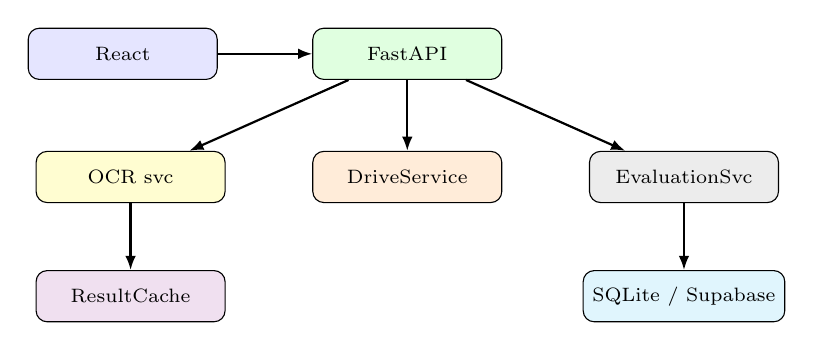
\begin{tikzpicture}[font=\scriptsize,
    box/.style={draw,rounded corners,minimum height=0.65cm,minimum width=2.4cm,align=center},
    arr/.style={-{Latex[length=1.8mm]},thick}]
    \node[box,fill=blue!10](fe){React};
    \node[box,fill=green!12,right=1.2cm of fe](api){FastAPI};
    \node[box,fill=orange!15,below=0.9cm of api](dr){DriveService};
    \node[box,fill=yellow!18,left=1.1cm of dr](ocr){OCR svc};
    \node[box,fill=gray!15,right=1.1cm of dr](ev){EvaluationSvc};
    \node[box,fill=violet!12,below=0.85cm of ocr](ca){ResultCache};
    \node[box,fill=cyan!12,below=0.85cm of ev](db){SQLite / Supabase};
    \draw[arr](fe)--(api);
    \draw[arr](api)--(dr);
    \draw[arr](api)--(ocr);
    \draw[arr](ocr)--(ca);
    \draw[arr](ev)--(db);
    \draw[arr](api)--(ev);
  \end{tikzpicture}

  \vspace{0.5em}
  \footnotesize
  Batch optimized path: download bytes $\rightarrow$ preprocess $\rightarrow$ Gemini OCR (dual Pro + vote) $\rightarrow$ \texttt{match\_and\_score} $\rightarrow$ cache row \texttt{sheet:v2:\{eval\}:\{file\}} $\rightarrow$ optional Drive rename + Sheets export.
\end{frame}

\begin{frame}{Service cheat-sheet (objective)}
  \tiny
  \begin{tabular}{@{}p{3.35cm}p{10.35cm}@{}}
    \toprule
    Module & Behavior \\
    \midrule
    \texttt{drive\_service.py} & OAuth SA or API key; list/download; batch rename. \\
    \texttt{pdf\_split\_service.py} & PDF $\rightarrow$ page JPEGs; \texttt{pdf:<sha>:pN} synthetic IDs for cache stability. \\
    \texttt{image\_preprocessing.py} & Paper crop + JPEG sizing before model POST. \\
    \texttt{ocr\_service.py} & Legacy single-image Gemini Flash stream. \\
    \texttt{optimized\_ocr\_service.py} / \texttt{multi\_region\_ocr\_service.py} & Pooled HTTP; load-aware endpoint pick. \\
    \texttt{answer\_key\_service.py} & Parse key files / vision-parse via Gemini. \\
    \texttt{evaluation\_service.py} & Pure \texttt{match\_and\_score}; SMCQ/MMCQ/NCQ + negatives. \\
    \texttt{batch\_evaluation\_service.py} & Parallel scoring over many OCR dicts; stats. \\
    \texttt{result\_cache\_service.py} & SQLite or Supabase; LRU; evaluation-scoped keys. \\
    \texttt{optimized\_database\_service.py} & WAL SQLite pool; batch inserts. \\
    \texttt{sheets\_service.py} & Match entry regex; write totals / per-Q / comments. \\
    \texttt{drive\_rename\_service.py} & Filename policy after grades (FUZZY-, UNMATCHED-, etc.). \\
    \bottomrule
  \end{tabular}
\end{frame}

% ===================== CODE EVALUATOR =====================
\section{Code evaluator deep dive}

\begin{frame}{Code evaluator: purpose}
  \small
  Grade \textbf{handwritten or photographed C solutions} per question using:
  \begin{itemize}
    \item Gemini/Vertex \textbf{vision OCR} to reconstruct C source from an image.
    \item \textbf{gcc} compile (\texttt{-c} object in FastAPI route; full link in \texttt{leetcode\_mode} harness).
    \item Optional LLM \textbf{syntax repair} (max 2 attempts) with strict \texttt{validate\_trivial\_fix} guardrails.
    \item \textbf{LeetCode-shaped test cases}: fetched via \texttt{leetcode\_mode} resolver \texttt{resolve\_leetcode\_problem\_and\_cases}, then executed in generated \texttt{main} harness per case.
  \end{itemize}
\end{frame}

\begin{frame}[fragile]{Evaluator bootstrap (\texttt{code\_eval\_endpoints.py})}
\begin{lstlisting}[style=py]
_vertex_key_path = str(Path(...) / "vertex_key.json")
if os.path.exists(_vertex_key_path):
    os.environ["GOOGLE_APPLICATION_CREDENTIALS"] = _vertex_key_path
    os.environ["GOOGLE_CLOUD_PROJECT"] = ... # from JSON project_id

sys.path.insert(0, ... / "c_code_evaluator")
from evaluate_c_from_image import extract_c_code_from_image, ...
from leetcode_mode import resolve_leetcode_problem_and_cases, evaluate_leetcode_cases
\end{lstlisting}
\vfill
\tiny Sets \texttt{GOOGLE\_CLOUD\_PROJECT} before importing modules that read it at import time.
\end{frame}

\begin{frame}[fragile]{HTTP surface (\texttt{code\_eval\_endpoints.py})}
\begin{lstlisting}[style=py]
router = APIRouter(prefix="/api/code-eval", tags=["code-evaluation"])

@router.post("/process-zip", response_model=CodeEvalResult)
async def process_zip_code_eval(file: UploadFile, answer_key: str = Form("")):
    # unzip images -> asyncio.to_thread(_process_single_image, ...)

@router.post("/process-drive-folder", response_model=CodeEvalResult)
async def process_drive_code_eval(request: DriveCodeEvalRequest):
    # DriveService.list_all_files_in_folder -> download -> same core processor
\end{lstlisting}
\end{frame}

\begin{frame}[fragile]{Answer key JSON for code eval}
\begin{lstlisting}[style=pys]
answer_key = {
  "problems": {
    "1": { "slug": "two-sum", "marks": 2 },
    "2": { "slug": "valid-parentheses", "marks": 1 }
  }
}
\end{lstlisting}
\vfill
\tiny \texttt{slug} is LeetCode \texttt{titleSlug}. Marks scale all-or-nothing per problem: all hidden examples must pass.
\end{frame}

\begin{frame}{\texttt{\_process\_single\_image}: step-by-step}
  \footnotesize
  \begin{enumerate}
    \item \textbf{Student identity}: Gemini vision JSON extract (\texttt{name}, \texttt{entry\_number}) with temperature 0; fallback regex from filename stem.
    \item \textbf{Code OCR}: call \texttt{extract\_c\_code\_from\_image} with image path and API key --- Vertex first if SA plus project, else API key.
    \item \textbf{Sanitize}: drop header lines matching Name / Entry Number markers from OCR noise.
    \item \textbf{Headers}: inject std includes if none present.
    \item \textbf{Compile}: run GCC compile-only pass (\texttt{-c}, \texttt{-std=c11}).
    \item \textbf{Repair loop}: up to two attempts of \texttt{fix\_ocr\_syntax\_errors} guarded by \texttt{validate\_trivial\_fix}.
    \item \textbf{Per problem}: \texttt{resolve\_leetcode\_problem\_and\_cases} then \texttt{evaluate\_leetcode\_cases}.
    \item \textbf{Score}: full marks only when every fetched testcase passes for that slug.
  \end{enumerate}
\end{frame}

\begin{frame}[fragile]{Student metadata micro-OCR (\texttt{code\_eval\_endpoints.py})}
\begin{lstlisting}[style=py]
prompt = (
    "Extract ONLY Name and Entry Number ... "
    "Return ONLY JSON with keys name and entry_number"
)
payload = {
    "contents": [{"role": "user", "parts": [
        {"text": prompt},
        {"inline_data": {"mime_type": mime_type, "data": base64_image}},
    ]}],
    "generationConfig": {"temperature": 0.0, "maxOutputTokens": 256},
}
model = os.environ.get("GEMINI_OCR_MODEL", "gemini-2.5-flash-lite")
\end{lstlisting}
\end{frame}

\begin{frame}[fragile]{\texttt{extract\_c\_code\_from\_image} (\texttt{evaluate\_c\_from\_image.py})}
\begin{lstlisting}[style=py]
prompt = (
    "You are doing OCR on a photo of handwritten/printed C source code.\n"
    "Return ONLY the reconstructed C code as plain text.\n"
    "- Do NOT add explanations.\n"
    "- Preserve newlines and indentation.\n"
)
payload = {
    "generationConfig": {"temperature": 0.0, "maxOutputTokens": 2048},
}
# Vertex stream if GOOGLE_APPLICATION_CREDENTIALS + project else GEMINI_API_KEY
return _strip_markdown_fences(raw)
\end{lstlisting}
\end{frame}

\begin{frame}[fragile]{\texttt{fix\_ocr\_syntax\_errors}: LLM repair contract}
\begin{lstlisting}[style=py]
prompt = (
    "Fix ONLY trivial OCR-induced syntax errors ... "
    "Do NOT change logic, algorithms, or control flow.\n"
    "ONLY fix: semicolons, brackets, OCR confusions 0/O, missing #include...\n"
    "Return ONLY the corrected C code.\n"
)
# Uses _vertex_generate_content or _gemini_generate_content (non-stream)
\end{lstlisting}
\end{frame}

\begin{frame}[fragile]{\texttt{validate\_trivial\_fix}: safety rails}
\begin{lstlisting}[style=py]
# Reject if >20 lines changed (SequenceMatcher opcodes)
# Reject if for/while/switch/goto/do counts change
# Reject disallowed new #includes (only stdlib whitelist)
# Reject if operator token sequence drifts beyond small edit budget
# Cap identifier rename drift (edit distance) bulk violations
return True, "accepted"
\end{lstlisting}
\vfill
\tiny Prevents ``fix'' pass from silently rewriting algorithms while repairing OCR typos.
\end{frame}

\begin{frame}[fragile]{ZIP ingestion implementation (\texttt{process\_zip\_code\_eval})}
\begin{lstlisting}[style=py]
with tempfile.TemporaryDirectory() as tmpdir:
    zip_path.write_bytes(await file.read())
    zf.extractall(extract_dir)
    image_files = sorted([p for p in extract_dir.rglob("*")
        if p.suffix.lower() in image_exts])
    for img in image_files:
        result = await asyncio.to_thread(
            _process_single_image, img, problems, work_dir, api_key)
\end{lstlisting}
\vfill
\tiny \texttt{asyncio.to\_thread} keeps FastAPI event loop responsive while CPU/gcc/Gemini-sync code runs in worker threads.
\end{frame}

\begin{frame}[fragile]{\texttt{\_compile\_c} in code-eval (syntax check)}
\begin{lstlisting}[style=py]
proc = subprocess.run(
    ["gcc", "-c", str(source_path), "-O2", "-std=c11", "-Wall", "-Wextra",
     "-o", str(binary_path)],
    capture_output=True, text=True, timeout=timeout_s,
)
\end{lstlisting}
\vfill
\tiny Object file proves compilation; actual LeetCode grading uses separate full-program harness compile (\texttt{leetcode\_mode.\_compile\_harness}) linking generated \texttt{main}.
\end{frame}

\begin{frame}[fragile]{Response model (\texttt{CodeEvalResult})}
\begin{lstlisting}[style=py]
class CodeEvalResult(BaseModel):
    total_students_processed: int
    results: List[Dict[str, Any]]
    errors: List[str]
\end{lstlisting}
\vfill
\tiny Each result dict mirrors objective-sheet scoring fields: \texttt{total\_score}, \texttt{details} with per-Q testcase counts, \texttt{comments} joining problem notes.
\end{frame}

\begin{frame}{Dual gcc roles (why two compile paths?)}
  \small
  \begin{itemize}
    \item \textbf{Endpoint \texttt{\_compile\_c}}: fast sanity check student OCR blob compiles as translation unit before wasting network on testcase fetch.
    \item \textbf{Harness compile}: each testcase wraps student functions + typed helpers + \texttt{main}; requires link-time symbols (\texttt{ListNode}, etc.).
    \item If sanity compile fails, repair agent runs; harness compile may still fail for unrelated reasons (unsupported signature).
  \end{itemize}
\end{frame}

\subsection{LeetCode testcase library (\texttt{leetcode\_mode.py})}

\begin{frame}{\texttt{resolve\_leetcode\_problem\_and\_cases}: merge strategy}
  \small
  \begin{enumerate}
    \item Optional \textbf{JSON file}: \texttt{\_parse\_cases\_file} --- embed \texttt{meta} + explicit \texttt{testcases} for air-gapped runs.
    \item Try \textbf{leetscrape family}: dynamic import \texttt{leetscrape} / \texttt{leetcode\_scrape} / \texttt{leetscraper}; probe \texttt{get\_problem}, \texttt{fetch\_problem}, etc.
    \item Try \textbf{pyleet}: \texttt{TestCaseRetriever} plus \texttt{get\_testcase} helpers.
    \item If still empty and \texttt{slug} set: \textbf{LeetCode GraphQL} \texttt{questionData} query --- parse \texttt{content} HTML for Input/Output pairs + \texttt{exampleTestcases} fallback.
    \item Drop cases without \texttt{expected}; \texttt{\_dedupe\_cases}; truncate to \texttt{max\_cases}.
  \end{enumerate}
\end{frame}

\begin{frame}[fragile]{GraphQL probe (\texttt{\_fetch\_from\_graphql})}
\begin{lstlisting}[style=py]
requests.post(
    "https://leetcode.com/graphql",
    json={"query": query, "variables": {"titleSlug": slug}},
    timeout=timeout_s,
)
# question.metaData JSON -> LeetProblemSpec (function name, param types)
# content HTML -> Input:/Output: regex pairs -> LeetCase args + expected
\end{lstlisting}
\vfill
\tiny Network dependency: institution firewall may block; use \texttt{cases\_file} fallback for exams.
\end{frame}

\begin{frame}{Datamodels (\texttt{leetcode\_mode.py})}
  \footnotesize
  \begin{tabular}{@{}p{3.4cm}p{10.4cm}@{}}
    \toprule
    Type & Meaning \\
    \midrule
    \texttt{LeetProblemSpec} & \texttt{function\_name}, param specs (name + logical type string), return type, sources list. \\
    \texttt{LeetCase} & \texttt{args} list (Python literals after parsing), \texttt{expected} value, \texttt{source} provenance tag. \\
    \texttt{CFunctionSpec} & Parsed C function signature from student OCR code via regex over bodies. \\
    \bottomrule
  \end{tabular}
\end{frame}

\begin{frame}{\texttt{evaluate\_leetcode\_cases}: execution model}
  \small
  \begin{enumerate}
    \item \texttt{extract\_c\_function\_specs} on OCR code --- find top-level functions; exclude \texttt{main}.
    \item \texttt{\_select\_function}: optional override, else match \texttt{problem.function\_name}, else single candidate / last resort heuristic with notes.
    \item For each case: \texttt{\_render\_case\_harness} builds C file with helper structs for \texttt{ListNode}/\texttt{TreeNode}, binds args by type (\texttt{int}, arrays, char*, 2D grids), adds \texttt{main} that prints normalized output.
    \item \texttt{gcc} full link harness $\rightarrow$ run binary $\rightarrow$ compare normalized stdout to expected string from \texttt{\_serialize\_expected}.
    \item Aggregate \texttt{PASSED} / \texttt{WRONG\_OUTPUT} / \texttt{TIMEOUT} / \texttt{COMPILE\_ERROR} / \texttt{HARNESS\_BUILD\_ERROR}.
  \end{enumerate}
\end{frame}

\begin{frame}[fragile]{Harness selection excerpt (\texttt{evaluate\_leetcode\_cases})}
\begin{lstlisting}[style=py]
specs = extract_c_function_specs(code)
selected, selection_notes = _select_function(
    specs,
    override_name=function_name_override,
    preferred_name=problem.function_name,
)
harness_code, expected_normalized = _render_case_harness(
    code=code, func=selected, problem=problem, case=case)
_compile_harness(harness_path, harness_bin, timeout_s=compile_timeout_s)
\end{lstlisting}
\end{frame}

\begin{frame}{Optional Python deps (grading machine)}
  \small
  \begin{itemize}
    \item \textbf{pyleet} --- programmatic official-style testcase tuples.
    \item \textbf{beautifulsoup4} --- cleaner HTML strip for GraphQL \texttt{content} parsing (regex fallback if missing).
    \item \textbf{leetscrape} ecosystem (optional; multiple module names tried).
    \item \textbf{gcc} system compiler --- required for any LeetCode harness run.
  \end{itemize}
\end{frame}

\begin{frame}[fragile]{\texttt{resolve\_leetcode\_problem\_and\_cases} signature}
\begin{lstlisting}[style=py]
def resolve_leetcode_problem_and_cases(
    *, slug: Optional[str], question_id: Optional[str],
    cases_file: Optional[Path], max_cases: int, timeout_s: int,
) -> Tuple[LeetProblemSpec, List[LeetCase], List[str]]:
    ...
\end{lstlisting}
\vfill
\tiny Returns merged problem spec (function name + param metadata), deduped cases with expectations, and diagnostic \texttt{notes} strings from each fetcher.
\end{frame}

\begin{frame}[fragile]{JSON testcase file format (\texttt{\_parse\_cases\_file})}
\begin{lstlisting}[style=pys]
{
  "title_slug": "two-sum",
  "meta": { "name": "twoSum", "params": [...], "return": {...} },
  "testcases": [
    { "args": [[2,7,11,15], 9], "expected": [0, 1] },
    { "input": "...", "output": "..." }
  ]
}
\end{lstlisting}
\end{frame}

\begin{frame}[fragile]{pyleet path (\texttt{\_fetch\_with\_pyleet})}
\begin{lstlisting}[style=py]
from pyleet import get_testcase
from pyleet.testcase_retriever import TestCaseRetriever

retriever = TestCaseRetriever()
question_data = retriever.get_question_data(resolved_slug)
meta = json.loads(question_data.get("metaData") or "{}")
pyleet_cases = get_testcase(title_slug=resolved_slug)
\end{lstlisting}
\vfill
\tiny Builds \texttt{LeetCase} objects by adapting tuple inputs to arg lists based on parameter count inference.
\end{frame}

\begin{frame}[fragile]{leetscrape dynamic import (\texttt{\_fetch\_with\_leetscrape})}
\begin{lstlisting}[style=py]
for module_name in ("leetscrape", "leetcode_scrape", "leetscraper"):
    module = importlib.import_module(module_name)
# Try get_problem / fetch_problem / get_question ... with slug kwargs
\end{lstlisting}
\vfill
\tiny Wide compatibility shim because PyPI package APIs differ; logs which module answered.
\end{frame}

\begin{frame}{\texttt{\_parse\_example\_pairs\_from\_content} (GraphQL HTML)}
  \small
  Regex scans stripped problem statement text for alternating \texttt{Input:} / \texttt{Output:} blocks; truncates at \texttt{Explanation:}.\\
  Fallback: split \texttt{exampleTestcases} / \texttt{sampleTestCase} newline blocks into synthetic cases (may lack expected $\rightarrow$ dropped later).
\end{frame}

\begin{frame}{Type-directed harness binding (\texttt{\_build\_input\_binding})}
  \footnotesize
  Maps Python literals from LeetCode cases to C declarations:
  \texttt{int} scalars, \texttt{bool}, C strings (\texttt{char buf[]}), int arrays (\texttt{int arr[] = \{...\}}), \texttt{char**} ragged strings, 2D grids with companion \texttt{colSizes}, linked lists via hidden \texttt{\_\_build\_listnode}, trees via \texttt{\_\_build\_tree} level-order arrays with null flags.
\end{frame}

\begin{frame}{Printed output conventions}
  \small
  Integer scalars: \texttt{printf} with width-aware format (\texttt{\%lld} for long long).\\
  Booleans: strings \texttt{true}/\texttt{false}.\\
  Arrays: bracketed comma-separated numbers.\\
  ListNode/TreeNode: bracketed level-order / adjacency walk matching LeetCode aesthetics for string compare.
\end{frame}

\begin{frame}[fragile]{Case verdict aggregation (\texttt{evaluate\_leetcode\_cases})}
\begin{lstlisting}[style=py]
matched = case_run_ok and (not case_timed_out) and (
    actual_normalized == expected_normalized)
if matched:
    status = "PASSED"; passed += 1
elif case_timed_out:
    status = "TIMEOUT"
elif not case_run_ok:
    status = "RUNTIME_ERROR"
else:
    status = "WRONG_OUTPUT"
\end{lstlisting}
\end{frame}

\begin{frame}{\texttt{c\_code\_evaluator/generate\_error\_images\_nanobanana.py}}
  \small
  Utility script for generating diagnostic/error imagery around evaluator tooling (batch helpers). Not on the hot HTTP path but part of developer ergonomics for debugging OCR failures.
\end{frame}

\section{Google Drive and Sheets}

\begin{frame}[fragile]{\texttt{drive\_service.py}: Drive API scope}
\begin{lstlisting}[style=py]
SCOPES = ['https://www.googleapis.com/auth/drive']
# Service account JSON preferred; else GOOGLE_API_KEY for public folders only
\end{lstlisting}
\end{frame}

\begin{frame}[fragile]{\texttt{sheets\_service.py}: entry detection}
\begin{lstlisting}[style=py]
ENTRY_NUMBER_PATTERN = re.compile(
    r'(\d{4})\s*([A-Za-z]{2,4})\s*(\d{2,5})',
)
# Header aliases for entry number, name, marks, comments columns
\end{lstlisting}
\end{frame}


\section{ZIP, PDF, Sheets publishing, and Evaluate UI}

\begin{frame}{Evaluate page: route and purpose}
  \small
  React route \texttt{/evaluate/:evaluationId} (\texttt{frontend-new-design/src/pages/evaluate/index.jsx}) --- faculty workflow for one quiz: load answer key, pick ingress (Drive / ZIP / PDF), run OCR pipeline, inspect results, sync/export to Google Sheets, optional Drive rename.
\end{frame}

\begin{frame}{Evaluate UI: layout and panels}
  \small
  Responsive grid (\texttt{lg:grid-cols-3}): left column stacks \textbf{Answer Key} panel and \textbf{OCR Pipeline} card; wider column for results table, stats, and logs.\\
  Objective vs \textbf{code} evaluations swap \texttt{AnswerKeyPanel} vs \texttt{CodeAnswerKeyPanel}.\\
  Shared Tailwind tokens: \texttt{bg-surface}, \texttt{border-border}, \texttt{text-text-primary}, semantic success/error callouts.
\end{frame}

\begin{frame}{Processing mode selector (frontend)}
  \small
  Segmented control with three modes:\\
  \textbf{Google Drive} --- folder URL input (\texttt{drive.google.com/drive/folders/...}).\\
  \textbf{ZIP Upload} --- dashed drop zone, \texttt{accept=".zip"}; expects answer key file + sheet images inside archive.\\
  \textbf{PDF} --- dashed drop zone \texttt{accept=".pdf"}; copy explains one student answer sheet per page, shared OCR/cache semantics with Drive.
\end{frame}

\begin{frame}{ZIP and PDF: client calls (\texttt{backendService.js})}
  \tiny
  \begin{itemize}\setlength\itemsep{0.12em}
    \item ZIP sync: \texttt{FormData} with \texttt{file}; optional query \texttt{force\_reprocess}, \texttt{extract\_answer\_key}; POST \texttt{/api/process-zip}.
    \item ZIP async: POST \texttt{/api/process-zip/start} $\rightarrow$ \texttt{run\_id}, poll \texttt{/api/pipeline-runs/\{id\}/status}.
    \item PDF async: \texttt{FormData} \texttt{file} + \texttt{evaluation\_id} (required helper \texttt{requireEvaluationId}); POST \texttt{/api/batch/process-pdf-optimized/start} $\rightarrow$ \texttt{processing\_id}, same poll as Drive batch.
    \item PDF sync: POST \texttt{/api/batch/process-pdf-optimized} $\rightarrow$ full \texttt{PipelineSummary} JSON.
  \end{itemize}
\end{frame}

\begin{frame}{Toolbar actions on Evaluate}
  \small
  \textbf{Sync from Sheet} --- pull master roster alignment / refresh cues from Google Sheets URL tied to course.\\
  \textbf{Export to Sheet} --- POST export pipeline with subsheet + evaluation name; surfaces success message including \texttt{studentResponse\_*} tab info when created.\\
  \textbf{Rename Drive files} --- batch rename after grading when folder URL present.\\
  Live \textbf{pipeline log} lines mirror OCR progress (percent, errors, cache hits).
\end{frame}

\begin{frame}{ZIP processing backend (\texttt{endpoints.py})}
  \small
  \texttt{POST /api/process-zip}: save upload $\rightarrow$ \texttt{\_process\_zip\_archive} extracts to temp tree $\rightarrow$ walk files into pseudo--Drive dicts (\texttt{id}=local path, \texttt{name}, \texttt{mimeType}, \texttt{local\_path}).\\
  \texttt{drive\_service.separate\_files} splits \textbf{answer key} candidates vs \textbf{student sheets} (filename heuristics).\\
  Answer key: first match parsed via \texttt{AnswerKeyService}; \texttt{extract\_answer\_key=false} skips ZIP key if server already holds key.\\
  Requires loaded answer key + at least one student sheet or returns 400/404 with actionable \texttt{detail}.
\end{frame}

\begin{frame}{ZIP background starter}
  \small
  \texttt{POST /api/process-zip/start}: persists zip bytes $\rightarrow$ creates SQLite pipeline run (\texttt{source\_type="zip"}, content-aware \texttt{source\_ref}) $\rightarrow$ \texttt{BackgroundTasks} runs \texttt{\_process\_zip\_archive\_background}.\\
  Response: \texttt{run\_id}, \texttt{status\_url} for UI polling --- mirrors long-running Drive batch ergonomics.
\end{frame}

\begin{frame}{PDF split service (\texttt{pdf\_split\_service.py})}
  \small
  PyMuPDF (\texttt{fitz}) renders each page to JPEG (default \textbf{220 DPI}, quality \textbf{90}) $\rightarrow$ balances checkbox legibility vs payload size.\\
  Full-file SHA-256 \texttt{pdf\_hash} for stable identity.\\
  Each page becomes a synthetic ``Drive-like'' dict: \texttt{id} = \texttt{pdf:<hash>:p<n>}, \texttt{local\_path}, \texttt{name}, \texttt{\_pdf\_meta} (\texttt{page\_number}, \texttt{pdf\_name}, hash).\\
  Same shape lets \texttt{\_process\_sheets\_optimized} consume PDF pages without a forked scorer.
\end{frame}

\begin{frame}{PDF batch orchestration (\texttt{batch\_endpoints\_optimized.py})}
  \small
  \texttt{\_run\_process\_pdf\_optimized}: status \texttt{splitting\_pdf} $\rightarrow$ \texttt{split\_pdf\_to\_pages} $\rightarrow$ assigns \texttt{processing\_id}, persists rendered JPEG dir (\texttt{pdf\_work\_dir}) for later \textbf{page image} HTTP downloads.\\
  Then invokes the \textbf{same} optimized multicolumn OCR + cache + scoring path used for Drive folders (including \texttt{evaluation\_id} scoping).\\
  Failure surfaces in \texttt{\_processing\_stats} with \texttt{ImportError} hint if PyMuPDF missing.
\end{frame}

\begin{frame}{PDF HTTP surface}
  \tiny
  \begin{itemize}\setlength\itemsep{0.1em}
    \item \texttt{POST /api/batch/process-pdf-optimized/start} --- multipart \texttt{file}, optional \texttt{evaluation\_id} form field; streams upload to temp with 1\,MiB chunks; returns \texttt{processing\_id}, \texttt{status\_url}, \texttt{mapping\_url}.
    \item \texttt{POST /api/batch/process-pdf-optimized} --- synchronous; returns \texttt{PipelineSummary} or 500 on split/pipeline failure.
    \item Follow-on: \texttt{/api/pdf-runs/\{id\}/mapping}, \texttt{.csv} export (optional \texttt{sheet\_url} for roster reconciliation), \texttt{/reconcile}, per-page image GET.
  \end{itemize}
\end{frame}

\begin{frame}{Google Sheets roles inside one spreadsheet}
  \small
  The product treats one Google Sheets URL as a \textbf{workbook hub}:\\[0.35em]
  \textbf{Master roster tab} --- canonical student rows (entry number + name); often named \texttt{student\_names} when URL omits \texttt{\#gid}.\\
  \textbf{Marks tab} (per quiz) --- created/updated by \texttt{update\_marks}; per-question columns + total + comments + statistics block.\\
  \textbf{Student response tab} --- \texttt{studentResponse\_\{quiz\}} with marked answers + answer-key row.\\
  \textbf{Super Sheet} tab --- one column per evaluation + cumulative total column for longitudinal grades.
\end{frame}

\begin{frame}{Reading the master sheet (\texttt{read\_student\_list})}
  \small
  Parses spreadsheet ID + optional gid/tab from URL.\\
  If no tab in URL: prefer tab titled \texttt{student\_names} (case-insensitive); else first sheet.\\
  Reads grid via \texttt{values().get}; \texttt{\_detect\_columns} maps headers to entry / name / marks / comments aliases.\\
  Builds \texttt{students} list with physical \texttt{row} indices for later writes.\\
  Side effect: caches roster in \texttt{\_master\_students\_cache} for rename fallback.
\end{frame}

\begin{frame}[fragile]{\texttt{GET /api/sheets/preview}}
  \small
  Non-destructive inspection: returns detected columns, chosen sheet name, full student list + count.\\
  Frontend \texttt{backendService.previewSheet(sheetUrl)} powers validation before export/sync.
\end{frame}

\begin{frame}{Writing marks (\texttt{update\_marks})}
  \tiny
  Reloads master students $\rightarrow$ smart-matches OCR results to roster rows $\rightarrow$ sorts rows \textbf{confident}, then \textbf{fuzzy}, then \textbf{unmatched}.\\
  Emits wide table: master entry/name, OCR entry + corrected entry, OCR name, each question score column, \texttt{SUM} formula total column, merged comments (fuzzy labels + name mismatch warnings).\\
  Appends \textbf{STATISTICS} block (mean, median, high, low via sheet formulas).\\
  Applies conditional formatting bands for fuzzy/unmatched via \texttt{\_format\_marks\_sheet}.
\end{frame}

\begin{frame}[fragile]{\texttt{POST /api/export-to-sheets}}
  \small
  Body: \texttt{ExportToSheetsRequest} (\texttt{sheet\_url}, optional \texttt{results}, \texttt{answer\_key}).\\
  Query: \texttt{subsheet\_name}, \texttt{evaluation\_name} (choose marks tab title).\\
  Resolution order for rows: request body \texttt{results} $\rightarrow$ in-memory \texttt{\_current\_results} $\rightarrow$ SQLite \texttt{students/results} legacy projection.\\
  Steps: (1) \texttt{update\_marks}; (2) if answer key + tab name --- \texttt{create\_student\_response\_sheet} as \texttt{studentResponse\_\{tab\}}; (3) \texttt{update\_super\_sheet} column for this evaluation.\\
  Returns aggregated summary JSON (per-step errors captured without failing entire export when optional steps fail).
\end{frame}

\begin{frame}{Student response tab layout}
  \small
  \texttt{create\_student\_response\_sheet}: columns \texttt{Name}, \texttt{Entry Number}, \texttt{Q1..Qn} from sorted answer-key ids; one row per student with \texttt{marked} text per question.\\
  Trailing blank row then \textbf{Answer Key} row (\texttt{USER\_ENTERED}); formatter bolds header + key row.\\
  Existing tab with same name is cleared then rewritten idempotently.
\end{frame}

\begin{frame}{Super Sheet longitudinal column}
  \small
  Tab name fixed: \texttt{Super Sheet}.\\
  If empty: seed headers \texttt{Entry Number | Name | \{evaluation\} | Cumulative Total}.\\
  If populated: insert new evaluation column before \texttt{Cumulative Total}, shift cells, recompute row-wise cumulative sums so multiple quizzes accumulate without manual pivoting.
\end{frame}

\begin{frame}[fragile]{\texttt{POST /api/export-student-responses}}
  \small
  Dedicated path when only the detailed response grid is needed (still requires answer key).\\
  Query \texttt{evaluation\_name}; optional body overrides for \texttt{results} / \texttt{answer\_key}.\\
  Delegates to \texttt{export\_responses\_to\_sheet} (service helper family alongside \texttt{create\_student\_response\_sheet}).
\end{frame}

\begin{frame}{Entry-number pattern (\texttt{sheets\_service})}
  \small
  \texttt{ENTRY\_NUMBER\_PATTERN} expects a four-digit year, a short branch code (letters), and a roll serial with flexible whitespace --- used when auto-detecting which master-sheet column holds official entry numbers.
\end{frame}

\begin{frame}{Design takeaway: one workbook, many surfaces}
  \small
  Faculty keep a \textbf{single} Spreadsheet ID in course metadata; the backend creates \emph{tabs} for different consumers (roster vs per-quiz marks vs item analysis vs cohort totals).\\
  Separating concerns avoids copying CSVs manually while still letting accountants open one familiar Google Sheets URL.
\end{frame}
\section{Throughput, fuzzy matching, and HTTP contracts}

\begin{frame}{Throughput section roadmap}
  \small
  \begin{enumerate}
    \item \textbf{Load shaping}: token buckets, round-robin regions, 429 cooldowns, dual OCR + tiebreaker (batch path).
    \item \textbf{Streaming pipeline}: bounded concurrency, DB writer queue, two-phase retries, cache tiers.
    \item \textbf{Fuzzy roster logic}: master-sheet vs OCR entry/name (\texttt{sheets\_service}).
    \item \textbf{Rename policy}: confident vs fuzzy vs unmatched filenames (\texttt{drive\_rename\_service}).
    \item \textbf{HTTP contracts}: Pydantic bodies, multipart ZIP, polling vs synchronous batch.
  \end{enumerate}
\end{frame}

\begin{frame}{Three OCR throughput backends (same Vertex idea, different orchestration)}
  \tiny
  \begin{tabular}{@{}p{3.2cm}p{11.4cm}@{}}
    \toprule
    Module & Role \\
    \midrule
    \texttt{multi\_region\_ocr\_service.py} & Many \texttt{(region, model)} endpoints (Flash / Flash-Lite / Pro); \texttt{LoadBalancer.get\_best\_endpoint()} scores load + latency + model priority + error rate. \\
    \texttt{optimized\_ocr\_service.py} & Prefer healthy Flash-Lite with lowest load; fallback endpoints; retries with backoff. \\
    \texttt{batch\_endpoints\_optimized.py} & \textbf{Pro-only} pool across regions; \textbf{token bucket RPM}; \textbf{round-robin}; \textbf{dual OCR} + third \textbf{majority} pass on disagreement. \\
    \bottomrule
  \end{tabular}
\end{frame}

\begin{frame}[fragile]{Load balancer score (\texttt{multi\_region\_ocr\_service.LoadBalancer})}
  \tiny
  Lower combined score wins among healthy endpoints under capacity.
\begin{lstlisting}[style=py]
def score_endpoint(ep):
    load_factor = ep.current_load / ep.max_concurrent
    time_factor = ep.avg_response_time / 2.0
    priority_factor = model_priority.get(ep.model, 4) / 4.0
    error_rate = ep.total_errors / max(ep.total_requests, 1)
    return load_factor + time_factor + priority_factor + error_rate
\end{lstlisting}
\vfill
\tiny If all saturated: pick least-loaded healthy; if none healthy: error path.
\end{frame}

\begin{frame}{Batch OCR endpoint pool (\texttt{\_ENDPOINT\_POOL})}
  \tiny
  Nine \texttt{gemini-2.5-pro} Vertex regions with RPM budgets (US clusters $\approx$ 250 RPM each; EU smaller). Combined intent: $\sim$2{,}250+ RPM headline capacity; stay on Pro for grading quality (no Flash fallback in this module).
\end{frame}

\begin{frame}[fragile]{Per-endpoint token bucket (\texttt{\_TokenBucket.acquire})}
  \footnotesize
  At most \texttt{rpm} tokens per 60s window: spacing $\approx$ \texttt{60.0 / rpm} seconds between grants (lock-held schedule).
\begin{lstlisting}[style=py]
async def acquire(self):
    async with self._lock:
        now = time.monotonic()
        wait = max(0.0, self._next_allowed - now)
        self._next_allowed = max(self._next_allowed, now) + self.interval
    if wait > 0:
        await asyncio.sleep(wait)
\end{lstlisting}
\end{frame}

\begin{frame}{Round-robin endpoint pick + 429 cooldown}
  \small
  \texttt{\_pick\_endpoint}: skip regions in exponential \textbf{cooldown} after HTTP 429; round-robin across remaining pool (global counter + lock).\\
  Cooldown: base 30s, doubles per repeat hit on same region, max 300s; successes clear cooldown counters for that region.
\end{frame}

\begin{frame}{Dual OCR and tiebreaker (batch)}
  \small
  \begin{enumerate}
    \item Two independent Pro OCR passes on \textbf{different regions}.
    \item If \texttt{answers} dicts agree on every question $\rightarrow$ accept.
    \item Any disagreement $\rightarrow$ third pass on fresh region; \textbf{majority vote} per question.
    \item Tiebreaker failure $\rightarrow$ majority of first two + warning tag in \texttt{comments}.
  \end{enumerate}
\end{frame}

\begin{frame}{Streaming pipeline: bounded concurrency}
  \small
  \texttt{PIPELINE\_MAX\_CONCURRENT} (default 24): semaphore around download+OCR+score so hundreds of files do not spawn hundreds of concurrent coroutines (OOM on 512MB hosts).\\
  \texttt{download\_sem}: caps Drive downloads vs OCR slots (\texttt{min(50, max(8, pipeline\_max * 2))}).
\end{frame}

\begin{frame}[fragile]{Background DB writer (pipelined commits)}
  \footnotesize
  Results enqueue to \texttt{asyncio.Queue}; worker flushes SQLite batches (every 20 rows or 2s idle); \texttt{None} sentinel ends run.
\begin{lstlisting}[style=py]
async def _db_writer_worker(queue, processing_id):
    batch = []
    while True:
        item = await asyncio.wait_for(queue.get(), timeout=2.0)
        if item is None:
            if batch:
                await batch_write_student_results(batch, ...)
            break
        batch.append(item)
        if len(batch) >= 20:
            await batch_write_student_results(batch, ...)
            batch = []
\end{lstlisting}
\end{frame}

\begin{frame}{Two-phase retry strategy (\texttt{\_process\_sheets\_optimized})}
  \small
  \textbf{Phase 1}: all sheets concurrent with bounded retries; empty entry / zero answers queue for phase 2 (does not block cohort).\\
  \textbf{Phase 2}: retries only failures with \textbf{fresh OCR} (cache bypass), quieter network after bulk completes.
\end{frame}

\begin{frame}{Cache tiers inside one cache row}
  \small
  Key pattern \texttt{sheet:v2:\{evaluation\_id\}:\{file\_id\}} stores JSON blobs:\\[0.4em]
  \begin{description}
    \item[Full eval hit] Valid \texttt{evaluation\_result}, sane entry, matching \texttt{answer\_key\_hash} $\rightarrow$ skip vision + scoring.
    \item[OCR-only hit] Valid \texttt{ocr\_result} $\rightarrow$ skip vision, still score.
    \item[Stale purge] Startup \texttt{purge\_stale\_for\_evaluation} removes rows whose hash differs from active key.
  \end{description}
\end{frame}

\begin{frame}[fragile]{\texttt{evaluation\_id} guard (cache isolation)}
  \footnotesize
  HTTP 400 if missing or literal \texttt{default} --- prevents cross-quiz cache bleed.
\begin{lstlisting}[style=py]
if not evaluation_id or evaluation_id.strip().lower() == "default":
    raise HTTPException(status_code=400,
        detail="evaluation_id is required ...")
\end{lstlisting}
\end{frame}

\begin{frame}{Shared HTTP session limits (\texttt{aiohttp})}
  \small
  One \texttt{ClientSession} per batch run with \texttt{TCPConnector(limit=256, limit\_per\_host=32, keepalive\_timeout=60)} so concurrent Vertex POSTs reuse connections without exhausting file descriptors.
\end{frame}

\begin{frame}{Fuzzy matching: where it applies}
  \small
  Sheets export correlates OCR rows with a master roster. \texttt{SheetsService.\_smart\_match\_score} outputs $[0,1]$ confidence from normalized entry edits + OCR-aware name similarity; exporter writes commentary consumed by \texttt{DriveRenameService.classify\_match}.
\end{frame}

\begin{frame}{Entry normalization before comparison}
  \small
  Sheet + OCR entries pass \texttt{\_correct\_entry\_number\_ocr}, strip non-alphanumerics, uppercase --- aligns formats like \texttt{2025 CSB 1454} vs OCR spacing noise.
\end{frame}

\begin{frame}{Smart match stages (\texttt{\_smart\_match\_score})}
  \tiny
  \begin{enumerate}\setlength\itemsep{0.12em}
    \item Exact corrected entry: 1.0 if name\_sim $\geq 0.40$ or OCR name empty; 0.98 if entry matches but names differ sharply.
    \item Year slide: same branch+roll, year within $\pm 3$, name\_sim $\geq 0.50$ $\rightarrow$ 0.95.
    \item Levenshtein $\leq 2$ on corrected entries + name\_sim $\geq 0.60$ $\rightarrow$ weighted blend capped 0.89.
    \item Raw-entry Levenshtein $\leq 2$ + name\_sim $\geq 0.50$ $\rightarrow$ capped 0.88 when corrector mangled tokens.
    \item Name-only rescue: name\_sim $\geq 0.90$ $\rightarrow$ up to 0.85 when roll handwriting unusable.
  \end{enumerate}
\end{frame}

\begin{frame}{Name similarity fusion (\texttt{\_name\_similarity})}
  \tiny
  Word overlap + fuzzy per-word Levenshtein ($\sim$30\% edits), substring containment bonus, bigram Jaccard on despaced strings, \texttt{difflib.SequenceMatcher} baseline. Weighted sum (words/bigrams/sequence/containment) clipped at 1.0.
\end{frame}

\begin{frame}{Rename classifier (\texttt{classify\_match})}
  \small
  Reads \texttt{comments} + entry:\\
  \texttt{fuzzy match} $\rightarrow$ fuzzy; \texttt{not found in master} / \texttt{absent} $\rightarrow$ unmatched; empty/\texttt{unknown}/\texttt{n/a} entry $\rightarrow$ unmatched; else confident.
\end{frame}

\begin{frame}{Drive filename templates}
  \tiny
  \begin{tabular}{@{}ll@{}}
    \toprule
    Category & Pattern \\
    \midrule
    confident & \texttt{\{Entry\} - \{Name\}.ext} \\
    fuzzy & \texttt{FUZZY - \{Entry\} - \{Name\}.ext} \\
    unmatched (OCR text) & \texttt{UNMATCHED - OCR \{entry\} - OCR \{name\}.ext} \\
    unmatched (no data) & \texttt{UNMATCHED\_NODATA - \{stem\}.ext} \\
    answer key & \texttt{ANSWER\_KEY - \{original\}.ext} \\
    error file & \texttt{ERROR - \{original\}.ext} \\
    \bottomrule
  \end{tabular}
\vfill
\tiny Duplicate entries append \texttt{ (DUP1)}, \texttt{ (DUP2)} after sanitization.
\end{frame}

\begin{frame}{Sanitization + skip rules}
  \small
  Replace unsafe filename chars; collapse whitespace; truncate length (50 chars default for student tokens).\\
  Optional \texttt{skip\_already\_renamed}: regex detects known prefixes (\texttt{FUZZY - }, \texttt{UNMATCHED}, \texttt{ANSWER\_KEY - }, \texttt{ERROR - }, roll-like prefix) to avoid rename churn on re-runs.
\end{frame}

\begin{frame}{Inline rename during batch (\texttt{\_rename\_one})}
  \small
  When \texttt{rename\_drive\_inline=True}: classify + compute target filename under async lock (duplicate counters); Drive API rename via \texttt{asyncio.to\_thread}; successful rename updates \texttt{file\_name}/\texttt{file\_id} on the result object for exports.
\end{frame}

\begin{frame}[fragile]{\texttt{RenameDriveFilesRequest}}
\begin{lstlisting}[style=pys]
class RenameDriveFilesRequest(BaseModel):
    folder_url: str
    dry_run: bool = False
    skip_already_renamed: bool = False
    results: Optional[List[Dict]] = None
    sheet_url: Optional[str] = None
\end{lstlisting}
\vfill
\tiny POST \texttt{/api/rename-drive-files}; \texttt{dry\_run} returns plan via \texttt{execute\_rename} without mutating Drive.
\end{frame}

\begin{frame}[fragile]{\texttt{ProcessFolderRequest}}
\begin{lstlisting}[style=pys]
class ProcessFolderRequest(BaseModel):
    folder_url: str
    evaluation_id: Optional[str] = None
    rename_drive_inline: bool = False
    group_multiple_pages: bool = False
\end{lstlisting}
\vfill
\tiny Powers \texttt{/api/batch/process-folder-optimized} (+ \texttt{/start}); server rejects blank/\texttt{default} evaluation ids before work begins.
\end{frame}

\begin{frame}[fragile]{\texttt{PipelineSummary}}
\begin{lstlisting}[style=pys]
class PipelineSummary(BaseModel):
    total_students_processed: int
    answer_key_source: str
    results: List[Any] = []
    errors: List[Dict] = []
    processing_stats: Dict = {}
\end{lstlisting}
\vfill
\tiny Typical synchronous batch completion payload; starters return ids for polling endpoints instead.
\end{frame}

\begin{frame}{Student row schema (\texttt{StudentResult})}
  \tiny
  Identity (\texttt{entry\_number}, \texttt{name}); aggregates (\texttt{total\_score}, \texttt{max\_score}, counts); \texttt{negative\_deduction}; \texttt{details} list of \texttt{QuestionResult} (\texttt{marked}, \texttt{correct}, \texttt{result}, \texttt{score}); \texttt{comments} carries fuzzy/absent markers; \texttt{file\_name}/\texttt{file\_id} bind Drive assets.
\end{frame}

\begin{frame}[fragile]{\texttt{AnswerKey} + \texttt{AnswerKeyEntry}}
\begin{lstlisting}[style=pys]
class AnswerKey(BaseModel):
    total_questions: int
    answers: Dict[int, AnswerKeyEntry]
    negative_marking: float = 0.0
    metadata: Dict = {}

class AnswerKeyEntry(BaseModel):
    question_type: str   # SMCQ, MMCQ, NCQ
    correct_answer: str
    positive_marks: float = 1.0
    negative_marks: float = 0.0
\end{lstlisting}
\end{frame}

\begin{frame}[fragile]{Sheets export models}
\begin{lstlisting}[style=pys]
class ExportToSheetsRequest(BaseModel):
    sheet_url: str
    results: Optional[List[Dict]] = None
    answer_key: Optional[Dict] = None

class SheetUpdateSummary(BaseModel):
    updated: int
    not_found: List[str] = []
    name_mismatches: List[Dict] = []
    errors: List[str] = []
\end{lstlisting}
\end{frame}

\begin{frame}[fragile]{Full pipeline models}
\begin{lstlisting}[style=pys]
class FullPipelineRequest(BaseModel):
    drive_folder_url: str
    sheets_url: str

class FullPipelineWithRenameRequest(BaseModel):
    drive_folder_url: str
    sheets_url: str
    rename_files: bool = True
    dry_run_rename: bool = False
\end{lstlisting}
\end{frame}

\begin{frame}[fragile]{Code-eval HTTP models}
\begin{lstlisting}[style=pys]
class CodeEvalRequest(BaseModel):
    answer_key: Dict[str, Any]

class DriveCodeEvalRequest(BaseModel):
    folder_url: str
    answer_key: Dict[str, Any]

class CodeEvalResult(BaseModel):
    total_students_processed: int
    results: List[Dict[str, Any]]
    errors: List[str]
\end{lstlisting}
\end{frame}

\begin{frame}{Multipart vs JSON FastAPI styles}
  \small
  \begin{description}
    \item[JSON] Body models (\texttt{ProcessFolderRequest}, \texttt{RenameDriveFilesRequest}, \texttt{DriveCodeEvalRequest}) with \texttt{application/json}.
    \item[Multipart] ZIP uploads (\texttt{UploadFile}) + optional form fields (\texttt{answer\_key} string).
    \item[Query] Flags such as \texttt{force\_reprocess}, destructive \texttt{confirm=true}, cache filters.
    \item[Paths] \texttt{/pipeline-runs/\{run\_id\}}, \texttt{/pdf-runs/\{id\}/mapping}, etc.
  \end{description}
\end{frame}

\begin{frame}{Synchronous batch vs background starter}
  \small
  \texttt{POST /api/batch/process-folder-optimized} awaits full pipeline $\rightarrow$ immediate \texttt{PipelineSummary}.\\
  \texttt{POST .../start} enqueues \texttt{BackgroundTasks}; HTTP returns \texttt{processing\_id}.\\
  Poll \texttt{GET /api/batch/processing-status/\{id\}} for processed counts, cache counters, error tails, partial snapshots.
\end{frame}

\begin{frame}{Representative JSON envelope}
  \tiny
  Mirrors \texttt{PipelineSummary}: counts, provenance string, \texttt{results} arrays (serialized \texttt{StudentResult}), structured \texttt{errors}, \texttt{processing\_stats} (\texttt{cache\_hits}, \texttt{ocr\_cache\_hits}, timing fields).\\
  Failure paths raise \texttt{HTTPException}(\texttt{detail=...}); validation errors include field paths via FastAPI/Pydantic.
\end{frame}

\begin{frame}{Cache DELETE endpoints (examples)}
  \tiny
  \begin{itemize}\setlength\itemsep{0.1em}
    \item \texttt{DELETE /api/cache/purge-evaluation/\{evaluation\_id\}}
    \item \texttt{DELETE /api/batch/purge-stale-eval-cache}
    \item \texttt{POST /api/cache/cleanup}, \texttt{POST /api/cache/clear} (legacy/global helpers with guards)
  \end{itemize}
\end{frame}

\begin{frame}{PDF run contracts (overview)}
  \tiny
  Multipart starter $\rightarrow$ \texttt{processing\_id};\\
  \texttt{GET /api/pdf-runs/\{id\}/mapping} + CSV export;\\
  \texttt{POST /api/pdf-runs/\{id\}/reconcile};\\
  binary page asset routes for QA viewers.
\end{frame}

\begin{frame}{Optimization cheat-sheet (objective batch)}
  \small
  \begin{itemize}
    \item Token buckets smooth Vertex quota usage ahead of 429 storms.
    \item Dual OCR + majority vote reduces single-model hallucinations.
    \item Semaphores cap RAM/FD on shared workers.
    \item Queue-backed SQLite writer amortizes disk writes during bursts.
    \item Full-eval cache avoids repeated vision when inputs unchanged.
    \item Phase-2 retries isolate pathological sheets without blocking everyone else.
  \end{itemize}
\end{frame}

% ===================== DATABASE / OCR condensed =====================
\section{OCR and migrations reference}

\begin{frame}{OCR-related module map (objective + utilities)}
  \tiny
  \begin{tabular}{@{}p{4.85cm}p{9.05cm}@{}}
    \toprule
    Module & Role \\
    \midrule
    \texttt{ocr\_service.py} & Legacy Gemini Flash stream per image. \\
    \texttt{optimized\_ocr\_service.py} / \texttt{multi\_region\_ocr\_service.py} & Pooled regional endpoints + load scoring. \\
    \texttt{image\_preprocessing.py} & Paper isolation + JPEG shrink before POST. \\
    \texttt{pdf\_split\_service.py} & Multi-page PDF $\rightarrow$ sheet-shaped dicts + stable hash IDs. \\
    \texttt{offline\_ocr\_service.py} & Tesseract/Paddle/EasyOCR without cloud. \\
    \texttt{extract\_text\_from\_images.py} & Repo-root script for quick Vertex image tests. \\
    \texttt{api/batch\_endpoints\_optimized.py} & Orchestrates dual OCR, cache, PDF runs. \\
    \bottomrule
  \end{tabular}
\end{frame}

\begin{frame}[fragile]{Migration \texttt{001\_result\_cache.sql} (core DDL)}
\begin{lstlisting}[style=py]
CREATE TABLE IF NOT EXISTS public.result_cache (
    file_hash         text PRIMARY KEY,
    file_name         text NOT NULL,
    ocr_result        jsonb NOT NULL,
    evaluation_result jsonb,
    answer_key_hash   text,
    created_at        timestamptz NOT NULL DEFAULT now(),
    last_accessed     timestamptz NOT NULL DEFAULT now(),
    access_count      integer NOT NULL DEFAULT 0,
    result_size       integer NOT NULL DEFAULT 0
);
ALTER TABLE public.result_cache ENABLE ROW LEVEL SECURITY;
\end{lstlisting}
\end{frame}

\begin{frame}[fragile]{Migration \texttt{002\_cache\_evaluation\_scope.sql}}
\begin{lstlisting}[style=py]
ALTER TABLE public.result_cache
    ADD COLUMN IF NOT EXISTS evaluation_id text,
    ADD COLUMN IF NOT EXISTS file_id       text;
CREATE INDEX IF NOT EXISTS idx_result_cache_eval_file
    ON public.result_cache(evaluation_id, file_id);
\end{lstlisting}
\end{frame}

\begin{frame}[fragile]{Migration \texttt{002\_pdf\_page\_map.sql}}
\begin{lstlisting}[style=py]
CREATE TABLE IF NOT EXISTS public.pdf_page_map (
    run_id          text NOT NULL,
    pdf_hash        text NOT NULL,
    page_number     integer NOT NULL,
    entry_number    text,
    name            text,
    status          text NOT NULL,
    total_score     numeric,
    max_score       numeric,
    PRIMARY KEY (run_id, page_number)
);
\end{lstlisting}
\end{frame}

\begin{frame}{SQLite (\texttt{database.py}) vs Supabase}
  \footnotesize
  SQLite: \texttt{students}, \texttt{submissions}, \texttt{results}.\\
  Supabase: \texttt{result\_cache} (JSONB OCR + eval), scoped by \texttt{evaluation\_id}/\texttt{file\_id}; \texttt{pdf\_page\_map} for PDF reconciliation.\\
  Cache PK: \texttt{sheet:v2:\{evaluation\_id\}:\{file\_id\}} consolidates OCR+eval rows.
\end{frame}

\begin{frame}[fragile]{\texttt{multi\_region\_ocr\_service}: load-aware scoring}
\begin{lstlisting}[style=py]
def score_endpoint(ep: OCREndpoint) -> float:
    load_factor = ep.current_load / ep.max_concurrent
    time_factor = ep.avg_response_time / 2.0
    priority_factor = self.model_priority.get(ep.model, 4) / 4.0
    error_rate = ep.total_errors / max(ep.total_requests, 1)
    return load_factor + time_factor + priority_factor + error_rate
\end{lstlisting}
\end{frame}

\begin{frame}[fragile]{\texttt{optimized\_ocr\_service}: tuning knobs}
\begin{lstlisting}[style=py]
self.max_image_size = (1920, 1920)
self.jpeg_quality = 85
self.optimal_batch_size = 25
self.connection_pool_size = 500
\end{lstlisting}
\end{frame}

\begin{frame}{Optimized batch OCR policy}
  \small
  Gemini 2.5 Pro only; dual independent OCR; disagree $\rightarrow$ third majority vote; token-bucket rate limiting; cache hit skips vision + scoring entirely (\texttt{batch\_endpoints\_optimized.py} module docstring).
\end{frame}

\begin{frame}[fragile]{\texttt{image\_preprocessing.preprocess\_for\_ocr}}
\begin{lstlisting}[style=py]
def preprocess_for_ocr(image_path: str,
    max_size: Tuple[int, int] = (1920, 1920),
    jpeg_quality: int = 85,
) -> Tuple[bytes, str]:
    """HSV paper crop -> resize -> JPEG bytes."""
\end{lstlisting}
\end{frame}

% ===================== CLOSING =====================
\section{Closing}

\section{Supplemental repository coverage}

\begin{frame}{\texttt{evaluation\_service.py}: scoring rules}
  \small
  Pure \texttt{match\_and\_score(answer\_key, student\_answers)} --- no LLM.\\
  Normalizes student option tokens; walks each keyed question; supports SMCQ/MMCQ/NCQ with per-question positive/negative marks plus global negative marking fallback.\\
  Treats \texttt{X}, \texttt{NONE}, \texttt{NA} style marks as unattempted (no negative).\\
  Emits \texttt{QuestionResult} rows (\texttt{marked}, \texttt{correct}, \texttt{result}, \texttt{score}) aggregated into \texttt{StudentResult}.
\end{frame}

\begin{frame}{\texttt{batch\_evaluation\_service.py}}
  \small
  Parallel-friendly wrappers around scoring (\texttt{batch\_match\_and\_score}, optimized answer-key preprocessing) for folder/ZIP throughput --- feeds bulk statistics surfaced in batch endpoints.
\end{frame}

\begin{frame}{\texttt{answer\_key\_service.py}: formats}
  \small
  \texttt{extract\_answer\_key(path, mime)} routes CSV/XLSX/PDF/image parsers; vision path uses Gemini Flash stream via Vertex SA or API key URL when structured parse fails.\\
  Normalizes into \texttt{AnswerKey} (\texttt{answers} dict of \texttt{AnswerKeyEntry}).\\
  Shared by ZIP ingestion, Drive extracts, and manual uploads.
\end{frame}

\begin{frame}{\texttt{drive\_service.py}: responsibilities}
  \small
  Service-account OAuth primary; optional API key mode for public folders.\\
  Folder ID extraction from URLs, recursive listing, MIME-aware downloads, batch rename orchestration, answer-key vs sheet separation heuristics (\texttt{separate\_files}).\\
  Batch rename batches HTTP calls with retry-friendly chunking (see \texttt{batch\_rename\_files}).
\end{frame}

\begin{frame}{\texttt{offline\_ocr\_service.py}}
  \small
  Local engines (\textbf{Tesseract}, \textbf{PaddleOCR}, \textbf{EasyOCR}) plus \textbf{ensemble} merge --- output shape matches cloud \texttt{extract\_objective\_sheet} so \texttt{match\_and\_score} stays unchanged.\\
  Heavy deps gated behind \texttt{requirements-local-ocr.txt}; lazy singletons amortize init cost.
\end{frame}

\begin{frame}{\texttt{cli.py}: headless pipeline}
  \tiny
  \texttt{python cli.py --drive-folder ... --sheet ...}\\
  Flags: \texttt{--mode offline|online}, \texttt{--local-ocr ensemble|paddle|tesseract|easyocr}, \texttt{--tab-name}, \texttt{--no-export}, dry-run options.\\
  Flow: enumerate Drive images $\rightarrow$ offline or Gemini OCR $\rightarrow$ \texttt{EvaluationService.match\_and\_score} $\rightarrow$ optional \texttt{SheetsService.update\_marks}.\\
  Useful for CI batches without SPA + complements Docker-hosted API.
\end{frame}

\begin{frame}{Deployment configs}
  \small
  \textbf{fly.toml}: Dockerfile build, internal port 8000, HTTPS, concurrency soft/hard limits, \texttt{/health} check, extended idle timeout for long OCR; comments document secrets (\texttt{SUPABASE\_DB\_URL}, base64 SA key).\\
  \textbf{railway.toml}: Nixpacks builder; \texttt{pip install -r backend/requirements.txt}; start via \texttt{/app/backend/start.sh}.
\end{frame}

\begin{frame}{Tests and utility scripts (repo root)}
  \tiny
  \texttt{backend/smoke\_test.py}, \texttt{backend/test\_phase3.py} --- manual sanity harnesses.\\
  \texttt{backend/test\_heic\_ocr.py}, repo \texttt{test\_heic\_ocr.py} --- image-format probes.\\
  \texttt{extract\_text\_from\_images.py} --- quick Vertex vision experiments.\\
  \texttt{frontend-new-design/test\_supabase\_auth.js}, \texttt{create\_test\_user.js} --- auth fixtures.\\
  Not wired into unified CI in this deck --- document presence for onboarding QA.
\end{frame}

\begin{frame}{\texttt{c\_code\_evaluator/} fixture files}
  \small
  Sample artifacts for offline exam bundles:\\
  \texttt{leetcode\_cases\_sample.json}, \texttt{testcases\_sample.json}, \texttt{testcases\_sample.txt}, \texttt{test\_expected.txt}, \texttt{test\_stdin.txt} --- illustrate JSON case format consumed by \texttt{leetcode\_mode} without hitting live GraphQL.\\
  Pair with \texttt{cases\_file} resolver strategy documented earlier.
\end{frame}

\begin{frame}{Documentation artifacts (not slides)}
  \small
  Root \texttt{README.md}, \texttt{IMPLEMENTATION\_SUMMARY.md}, \texttt{frontend-new-design/IMPLEMENTATION\_PLAN.md}, \texttt{REFINED\_PLAN.md}, \texttt{c\_code\_evaluator/README.md} capture historical decisions --- treat as companion reading to this PDF.
\end{frame}


\begin{frame}{Screenshot placeholder --- Evaluate UI}
  \begin{center}
    \fbox{\parbox{0.9\textwidth}{\centering\vspace{1.5cm}
      \textit{Browser: \texttt{/evaluate/:evaluationId}}\vspace{1.5cm}}}
  \end{center}
\end{frame}

\begin{frame}{Screenshot placeholder --- IDE / Supabase}
  \begin{center}
    \fbox{\parbox{0.9\textwidth}{\centering\vspace{1.5cm}
      \textit{\texttt{batch\_endpoints\_optimized.py} or Supabase \texttt{result\_cache} table}\vspace{1.5cm}}}
  \end{center}
\end{frame}

\begin{frame}{Cross-cutting themes (still this single deck)}
  \small
  Observability (trace IDs), fair grading (blind mode), schema versioning (answer-key JSON), retention/purge on Supabase cache tables.
\end{frame}

\begin{frame}{Future work (selected)}
  \small
  \begin{itemize}
    \item Signed JWT between FE and BE; org-level quotas.
    \item Pin LeetCode testcase bundles per exam (\texttt{cases\_file}) for reproducibility offline.
    \item Sandboxed execution (Docker/seccomp) instead of raw \texttt{gcc} on shared hosts.
    \item Golden OCR + golden LeetCode harness regression CI.
    \item Model routing dashboard (cost vs accuracy).
  \end{itemize}
\end{frame}

\begin{frame}{Build}
  \centering
  \texttt{pdflatex presentation3\_future\_development.tex}
\end{frame}

\end{document}
